% Created 2016-08-17 Wed 14:38
\documentclass[tikz]{standalone}

\usepackage[utf8]{inputenc}
\usepackage[T1]{fontenc}

\usepackage{circledsteps}

\RequirePackage{xcolor}

%% HPI color definitions according to the design manual
% These do not exactly match the RGB values used in the Powerpoint slide master due to unknown reasons
\definecolor{hpiyellow}{RGB}{246,168,0}
\definecolor{hpiorange}{RGB}{221,97,8}
\definecolor{hpired}{RGB}{177,6,58}
\definecolor{hpigray}{RGB}{90,96,101}
\definecolor{hpiblue}{RGB}{0,122,158}


\renewcommand{\sfdefault}{neosans}
% Different font weights for neosans
\newcommand{\textl}[1]{{\fontseries{l}\selectfont #1}} % light
\newcommand{\textm}[1]{{\fontseries{m}\selectfont #1}} % medium, same as default weight
\newcommand{\textsb}[1]{{\fontseries{sb}\selectfont #1}} % semibold
\newcommand{\textmb}[1]{{\fontseries{mb}\selectfont #1}} % bold, same as \textbf
\newcommand{\texteb}[1]{{\fontseries{eb}\selectfont #1}} % extra bold
\newcommand{\textub}[1]{{\fontseries{ub}\selectfont #1}} % ultra bold

\tikzset{every picture/.style={/utils/exec={\sffamily}}}
\tikzset{flipflop RSflanke/.style={
  flipflop,
  flipflop def={t1=S, t2=C, c2=1, t3=R, t6=Q, t4={\ctikztextnot{Q}}}
}}


\tikzset{
  mechanicalSwitch/.pic={
    \coordinate (-inUp) at (135:2); 
    \coordinate (-inDown) at (235:2);
    \coordinate (-out) at (2,0);
    \coordinate (-center) at (0,0);
    
    \draw (0,0) circle [radius = 2cm];
    \draw [fill=gray!20] (0,0) circle [radius = 0.2cm];

    \draw (0, 0) -- (2, 0);
    \draw (135:.8) -- (135:2); 
    \draw (225:.8) -- (225:2); 

    \draw [fill=gray!20] (2, 0) circle [radius=0.05cm]; 
    \draw [fill=gray!20] (135:2) circle [radius=0.05cm]; 
    \draw [fill=gray!20] (225:2) circle [radius=0.05cm]; 

    
    \draw [thick] (0,0) -- (175:1.5); 

    \draw [dashed, <->, domain=135:225] plot ({cos(\x)}, {sin(\x)}); 
  },
  mechanicalSwitchClosed/.pic={
    \coordinate (-inUp) at (135:2); 
    \coordinate (-inDown) at (255:2);
    \coordinate (-out) at (2,0);
    \coordinate (-center) at (0,0);
    \draw (0,0) circle [radius = 2cm];
    \draw [fill=gray!20] (0,0) circle [radius = 0.2cm];

    \draw (0, 0) -- (2, 0);
    \draw (135:.8) -- (135:2); 
    \draw (225:.8) -- (225:2); 

    \draw [fill=gray!20] (2, 0) circle [radius=0.05cm]; 
    \draw [fill=gray!20] (135:2) circle [radius=0.05cm]; 
    \draw [fill=gray!20] (225:2) circle [radius=0.05cm]; 

    
    \draw [thick] (0,0) -- (135:2); 

    \draw [dashed, <->, domain=135:225] plot ({cos(\x)}, {sin(\x)}); 
  }
}


\usetikzlibrary{calc}
\usetikzlibrary{positioning}


\usetikzlibrary{shapes.callouts}
\usetikzlibrary{decorations.pathreplacing,decorations.pathmorphing,decorations.shapes,decorations.markings,calc,spy}


\begin{document}

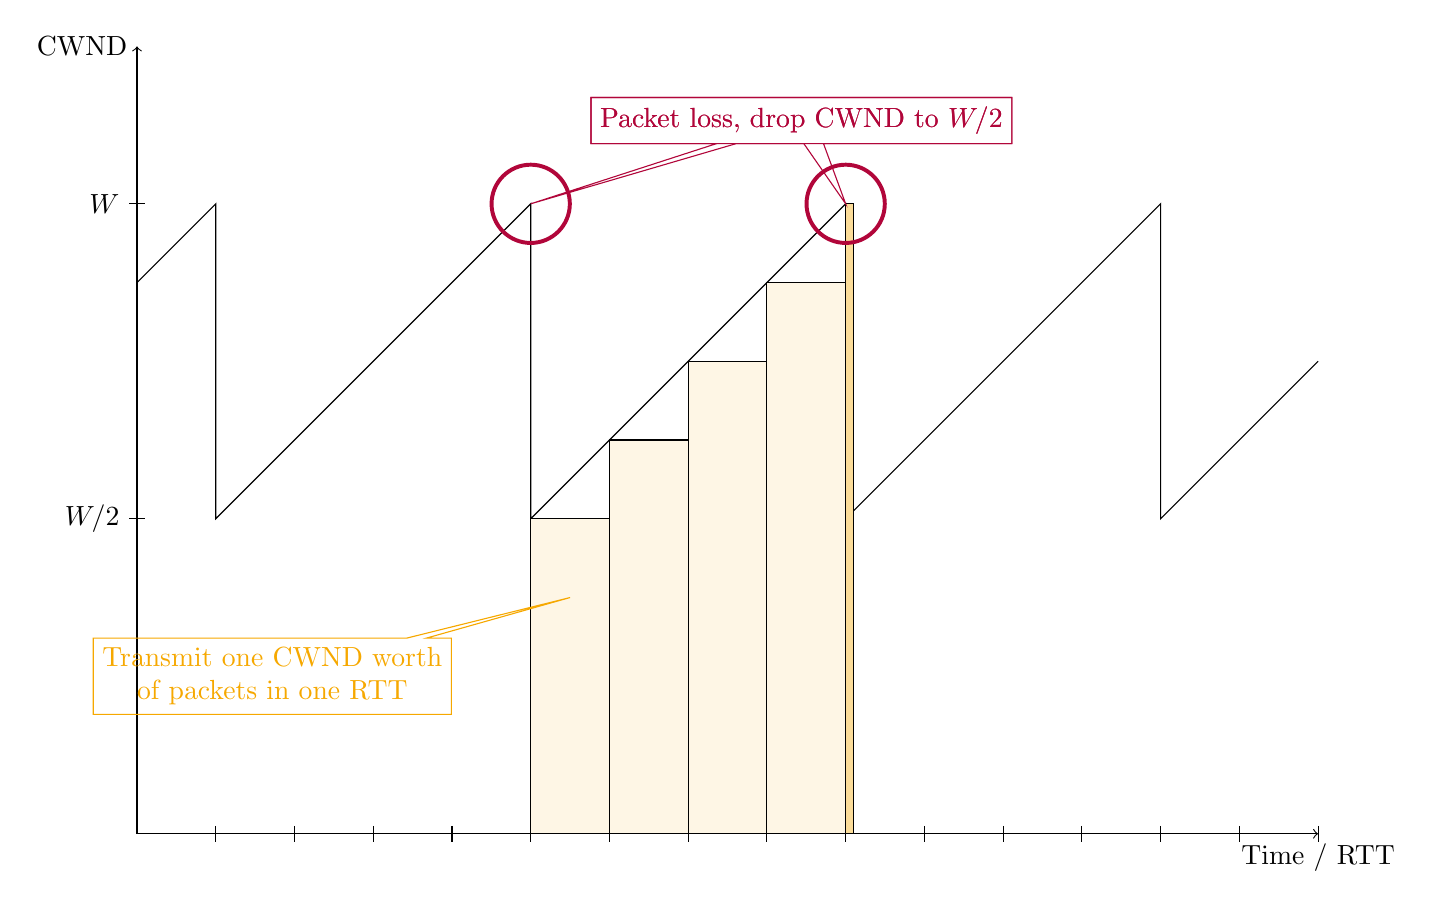
\begin{tikzpicture}
  \draw [->] (0,0) -- (0, 10) node [left] {CWND};
  \draw (0.1,8) -- (-0.1,8) node [left] {$W$};
  \draw (0.1,4) -- (-0.1,4) node [left] {$W/2$};

  \draw [->] (0,0) -- (15, 0) node [below] {Time / RTT}; 

  \foreach \i in {1,...,15} {
    \draw (\i, 0.1) -- (\i, -0.1); 
  }

  % basic process
  \draw (0,7) -- (1,8) -- (1,4) -- (5,8) -- (5,4) -- (9,8) -- (9,4) -- (13, 8) -- (13, 4) -- (15, 6);

  \foreach \i in {5,6,7,8} {
    \draw [fill=hpiyellow!10] (\i,0) rectangle (\i+1,\i-1); 
  }
  \draw [fill=hpiyellow!40] (9,0) rectangle (9.1,8); 

  % show packet losses: 
  \node [circle, draw, hpired, scale=3, line width=0.5mm] at (5,8) (pl) {};
  \node [circle, draw, hpired, scale=3, line width=0.5mm] at (9,8) (pl2) {};
  \node [draw, hpired, rectangle callout, callout absolute pointer={(pl)}, above right=0.5 of pl] {Packet loss, drop CWND to $W/2$}; 
  \node [draw, hpired, rectangle callout, callout absolute pointer={(pl2)}, above right=0.5 of pl] {Packet loss, drop CWND to $W/2$}; 

  \node [draw, hpiyellow, rectangle callout, align=center, 
  callout absolute pointer={(5.5, 3)}, anchor=east] at (4,2) {Transmit one CWND worth\\ of packets in one RTT};

  
  
\end{tikzpicture}

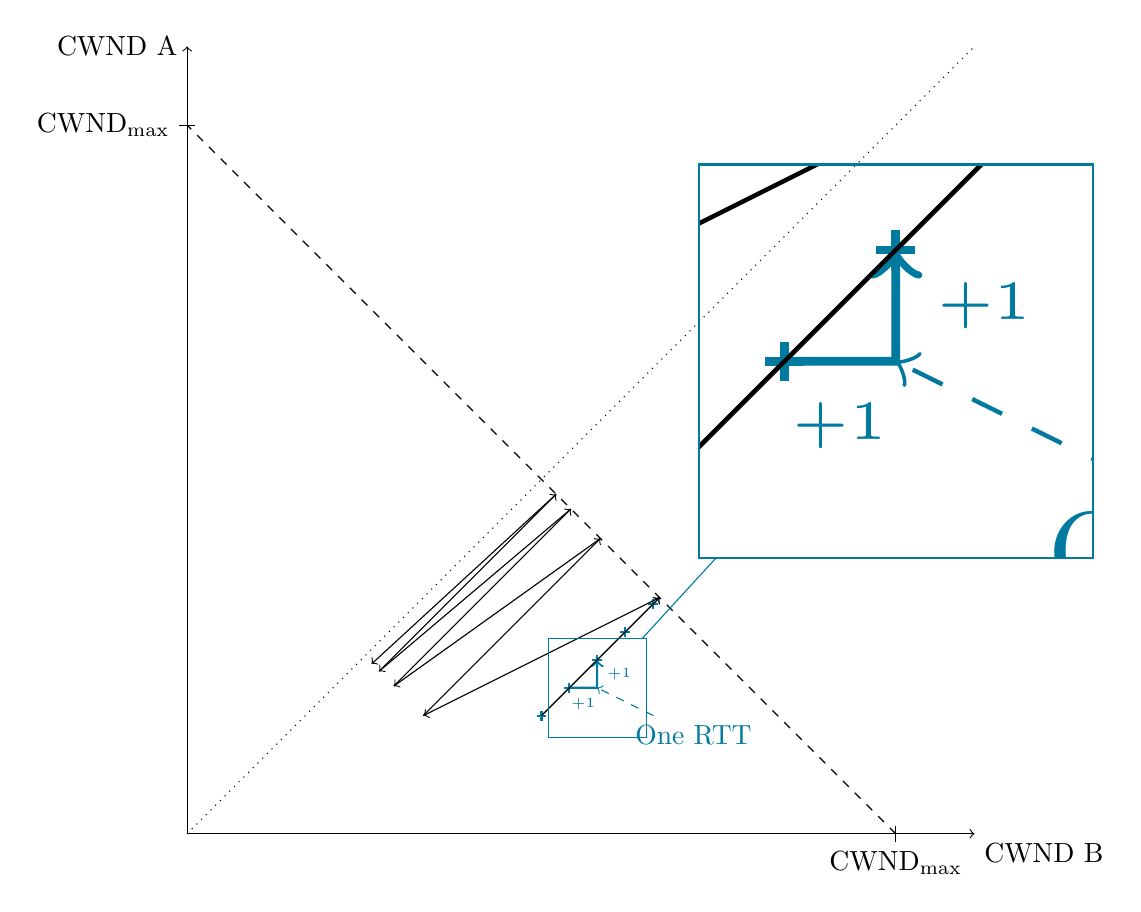
\begin{tikzpicture}[spy using outlines={magnification=4, size=5cm, connect spies}]
  \draw [->] (0,0) -- (0, 10) node [left] {CWND A};
  \draw [->] (0,0) -- (10, 0) node [below right] {CWND B}; 

  % \pause 
  \draw (0.1,9) -- (-0.1,9) node [left] {$\mathrm{CWND}_\mathrm{max}$}; 
  \draw (9, 0.1) -- (9, -0.1) node [below] {$\mathrm{CWND}_\mathrm{max}$};
  % \pause 
  \draw [dotted] (0,0) -- (10,10);

  % \pause 
  \draw [dashed] (9,0) -- (0,9);
  % \pause 

  % first iteration:
  \draw [->] (4.5, 1.5) to (6, 3); 
  % \pause 
  \draw [decorate, thick, decoration={crosses, segment length=5mm}, hpiblue] (4.5, 1.5) to (6, 3); 

  % \pause 
  \draw [decorate,
  decoration={markings,
    mark=at position 5mm with {
      \draw [thick, hpiblue,->] (0,0) to node [below, rotate=0] {\tiny +1}
      (0.5*5mm,-0.5*5mm) node (n0) {} node [below right=0.5] (n1) {One RTT}
      to node [right, rotate=0] {\tiny +1}  
      (5mm, 0);
      \draw [thin, dashed, hpiblue, ->] (n1) -- (0.5*5mm,-0.5*5mm); 
    }
  }
  ] (4.5, 1.5) to (6,3); 

  % \pause

  \spy [hpiblue] on (n0) in node at (9,6); 
  
  % \pause 
  
  \foreach \a/\b [remember=\a as \lasta (initially 4.5),
  remember=\b as \lastb (initially 1.5),
  ] in {6/3,3/1.5, 5.25/3.75, 2.625/1.875, 4.875/4.125, 2.4375/2.0625, 4.6875/4.3125, 2.34275/2.15625} {
    \draw [->] (\lasta, \lastb)  -- (\a, \b); 
    % \pause 
  }

  % \pause
  
  
  % % \pause 
  % \foreach \a/\b [count=\i, remember=\a as \lasta (initially 3.75),
  % remember=\b as \lastb (initially 0.75),
  % ] in {3/1.5,  2.625/1.875, 2.4375/2.0625, 2.34275/2.15625} {
  % \draw [decorate, decoration={brace, raise=5pt}] (\lasta, \lastb) to node[below left=1pt] (rtt\i) {}  (\a, \b); 
  % }


  %   \node (rttlabel) at (1,0.5)  {One RTT}; 
  %   \foreach \i in {1,...,4} {
  %   %   \node [draw, rectangle callout,
  %   %   callout absolute pointer={(rtt\i)}] at (1,0.5) {One RTT};
  %   \draw [->] (rttlabel) -- (rtt\i); 
  % }

\end{tikzpicture}






\end{document}